\documentclass[conference]{IEEEtran}

\usepackage{amsmath,amssymb}
\usepackage{graphicx}
\usepackage{booktabs}
\usepackage{multirow}
\usepackage{array}
\usepackage{xcolor}
\usepackage{textcomp}
\usepackage{tikz}
\usepackage{pgfplots}
\usepackage[hidelinks]{hyperref}
\usetikzlibrary{positioning,fit,arrows.meta,backgrounds}
\pgfplotsset{compat=1.16}

\definecolor{navy}{HTML}{0F2B40}
\definecolor{okorange}{HTML}{E8832A}
\definecolor{okgreen}{HTML}{2F8F5B}
\definecolor{mint}{HTML}{E3F2E9}
\definecolor{peach}{HTML}{FDEFD9}

\newcommand{\IdleShare}{63}
\newcommand{\IdleShareStress}{46}
\newcommand{\NSeeds}{50}
\newcommand{\HeadlineW}{1.5}
\newcommand{\FusedCO}{12.9}
\newcommand{\FusedCOci}{1.2}
\newcommand{\FusedCOStress}{2.4}
\newcommand{\FusedLatCut}{81}
\newcommand{\NetLatCut}{83}
\newcommand{\NetCO}{1.7}
\newcommand{\FusedLatCutStress}{54}
\newcommand{\NetLatCutStress}{56}
\newcommand{\FusedLowW}{5.2}
\newcommand{\EnergyOnlyCO}{7.3}
\newcommand{\FusedDecisionUs}{3.4}
\newcommand{\NSystemsScraped}{1118}
\newcommand{\NSystemsKept}{1115}
\newcommand{\NRowsKept}{12{,}265}
\newcommand{\YearLo}{2007}
\newcommand{\YearHi}{2026}
\newcommand{\MapeXgb}{12.0}
\newcommand{\MapeOracle}{7.7}
\newcommand{\MapePlaceholder}{65}
\newcommand{\MapeTemporal}{26}
\newcommand{\TrainSystems}{800}
\newcommand{\TestSystems}{315}
\newcommand{\SmallIdle}{32}
\newcommand{\SmallHalf}{59}
\newcommand{\SmallPeak}{89}


\hyphenation{Okube SPECpower}

\begin{document}

% ---------------------------------------------------------------- cover page
\begin{titlepage}
\centering
\vspace*{2.2cm}
{\normalsize Course Project Report on}\\[8pt]
{\Large\bfseries OKUBE-ENERGY}\\[10pt]
{\normalsize Submitted in partial fulfillment of the requirements for the degree of}\\[10pt]
{\normalsize BACHELOR OF TECHNOLOGY}\\[2pt]
{\normalsize in}\\[2pt]
{\normalsize INFORMATION TECHNOLOGY}\\[2pt]
{\normalsize by}\\[8pt]
{\normalsize\bfseries Sanchit Srisha Udupa (231IT060)}\\[2pt]
{\normalsize\bfseries Aditi Pandey (231IT003)}\\[12pt]
{\normalsize\itshape under the guidance of}\\[8pt]
{\large\bfseries Dr. Bhawana Rudra}\\[26pt]

\includegraphics[width=4.2cm]{figures/nitk_logo.png}\\[26pt]
{\normalsize DEPARTMENT OF INFORMATION TECHNOLOGY}\\[2pt]
{\normalsize NATIONAL INSTITUTE OF TECHNOLOGY KARNATAKA}\\[2pt]
{\normalsize SURATHKAL, MANGALORE - 575025}\\[14pt]
{\normalsize October, 2026}
\end{titlepage}

% ---------------------------------------------------------------- front matter
\title{Okube-Energy: Fusing Network and Carbon Cost\\in a Custom Container Scheduler}

\author{\IEEEauthorblockN{Sanchit Srisha Udupa}
\IEEEauthorblockA{\textit{Department of Information Technology}\\
\textit{NIT-Surathkal}\\
Surathkal, Mangalore, India\\
sanchit.231it060@nitk.edu.in}
\and
\IEEEauthorblockN{Aditi Pandey}
\IEEEauthorblockA{\textit{Department of Information Technology}\\
\textit{NIT-Surathkal}\\
Surathkal, Mangalore, India\\
aditip.231it003@nitk.edu.in}}

\maketitle

\begin{abstract}
Container orchestrators place workloads mainly by resource availability and treat network topology and carbon cost as secondary. We present Okube-Energy, a scheduler extension for Okube, a custom Go orchestrator, that scores every candidate node on network cost and carbon cost in one pipeline. Its novelty lies in four things: a composable pipeline in which the network and energy stages toggle independently, so the default, network-only, energy-only and fused schedulers are ablations of one code path; a task-class-aware carbon weight that is raised for time-flexible work and lowered for latency-critical work; a carbon cost on a fixed scale, which treats a zero-carbon grid as a valid value and does not inflate differences between uniformly clean grids; and an evaluation that computes CO$_2$ from power curves learned from \NSystemsKept{} SPECpower\_ssj2008 systems. On a seeded simulation of a three-zone cluster, with settings chosen on one set of seeds and reported on another, the fused scheduler at an energy weight of \HeadlineW{} cuts dynamic CO$_2$ by \FusedCO\% (95\% CI $\pm\FusedCOci$) against the default scheduler while keeping mean dependency latency \FusedLatCut\% below default (network-aware alone: \NetLatCut\%). Under a saturating workload the carbon gain shrinks to \FusedCOStress\%. The study is simulation-based and uses illustrative regional carbon intensities; its limits are stated in Section~\ref{sec:threats}.
\end{abstract}

\begin{IEEEkeywords}
container orchestration, scheduler, network-aware scheduling, carbon-aware computing, power model, SPECpower, carbon intensity, Go
\end{IEEEkeywords}

% ---------------------------------------------------------------- I. Introduction
\section{Introduction}
A container orchestrator decides which node runs each task. The default Kubernetes scheduler ranks nodes by resource fit: whether a node has enough CPU, memory and disk, and how balanced the resulting utilisation is. Two costs are largely absent from that model. The first is \emph{network cost}: services that depend on each other pay inter-service latency when placed far apart, and tail latency degrades even when every node is well provisioned. The second is \emph{carbon cost}: the same task draws different energy on different nodes, and the electricity behind each node has a different carbon intensity, so a resource-optimal placement is often not a carbon-optimal one.

Prior work treats these costs separately. Diktyo \cite{santos2023} makes placement network-aware but is carbon-blind. Piontek et al.\ \cite{piontek2024} separate latency-critical from time-shiftable jobs and move the latter to lower-carbon windows, but have no network model and rely on a simple moving-average forecast. Saad et al.\ \cite{saad2025} predict per-workload energy with federated learning on top of Kepler \cite{amaral2023}, but stop at prediction and make no scheduling decision.

This paper builds the missing combination inside Okube, a custom manager/worker orchestrator written in Go with Docker execution and etcd coordination. We deliberately did not write a Kubernetes plugin: a custom scheduler lets us change placement logic end to end, and the same pipeline code is driven unchanged by an offline simulator.

\subsection{Novelty and contributions}
\label{sec:novelty}
Table~\ref{tab:positioning} positions this work against the three papers above. The contributions are:
\begin{enumerate}
\item \textbf{One pipeline, four schedulers.} Network scoring and energy scoring are independent stages of a single pipeline. The default, network-only, energy-only and fused schedulers differ only in two flags, so any difference between them is attributable to a stage and not to a different implementation. An energy weight of zero reproduces the network-only scores exactly, which a regression test enforces.
\item \textbf{Class-aware fusion.} The carbon weight is scaled by task class ($\times0.35$ critical or urgent, $\times1.4$ flexible). This adapts the critical/shiftable distinction of \cite{piontek2024} from \emph{when} to \emph{where}, and combines it with a Diktyo-style \cite{santos2023} network cost.
\item \textbf{A carbon cost on a fixed scale.} Our first formulation min--max normalised the energy cost across the candidates. That stretches any spread to the full range, so a $15$\,g/kWh node looked as bad as it could be next to a $0$\,g/kWh node. Scoring against a fixed reference intensity removes this failure, and an explicit ``unknown'' replaces the sentinel that made a real zero look unset.
\item \textbf{Power curves learned from open data.} We scraped the SPECpower\_ssj2008 published results (\NSystemsScraped{} systems with full load curves) and trained a monotone gradient-boosted model from hardware to watts. It replaces a made-up idle/max pair whose error was \MapePlaceholder\% by one with \MapeXgb\% held-out error.
\item \textbf{A reproducible, paired evaluation.} A seeded simulator drives the real scheduler code. Settings are chosen on one seed range and results reported on a disjoint one, with paired comparisons and confidence intervals.
\end{enumerate}
Our headline finding is that the fused scheduler keeps nearly all of the network latency gain while delivering a carbon reduction that the network-aware scheduler alone does not. We also report where that gain disappears and which parts of the comparison are not as clean as they first appear (Section~\ref{sec:discussion}).

\begin{table*}[t]
\centering
\caption{Positioning against the closest prior work, based on each paper's stated scope.}
\label{tab:positioning}
\small
\begin{tabular}{@{}lccccc@{}}
\toprule
 & Network-aware & Carbon / energy signal & Job-class aware & Learned power model & Fused, with ablations \\
\midrule
Diktyo \cite{santos2023}            & \checkmark & $\times$ & $\times$ & $\times$ & $\times$ \\
Piontek et al.\ \cite{piontek2024}  & $\times$ & \checkmark (moving average) & \checkmark (when) & $\times$ & $\times$ \\
Saad et al.\ \cite{saad2025}        & $\times$ & \checkmark (federated prediction) & $\times$ & \checkmark & $\times$ \\
\textbf{Okube-Energy (this work)}   & \checkmark & \checkmark (regional intensity) & \checkmark (where) & \checkmark (single model) & \checkmark \\
\bottomrule
\end{tabular}
\end{table*}

The rest of the paper is organised as follows. Section~\ref{sec:related} reviews related work, Section~\ref{sec:arch} describes the architecture, Section~\ref{sec:model} the scoring model, Section~\ref{sec:data} the data and power model, Section~\ref{sec:eval} the evaluation method, Section~\ref{sec:results} the results, and Sections~\ref{sec:discussion}--\ref{sec:future} the discussion, threats, conclusion and future work.

% ---------------------------------------------------------------- II. Related work
\section{Background and Related Work}
\label{sec:related}
\textbf{Network-aware scheduling.} Diktyo \cite{santos2023} models an application as a dependency graph and places services to reduce latency and respect bandwidth, reporting large latency reductions against the default Kubernetes scheduler. We adopt its idea of costing a node by the latency to the nodes hosting a service's dependencies.

\textbf{Carbon-aware scheduling.} Piontek et al.\ \cite{piontek2024} classify jobs as critical or shiftable and delay the latter into lower-carbon windows, using a weighted moving average to forecast carbon. A recent survey \cite{survey2025} covers the wider space of carbon-aware container scheduling. These systems choose \emph{when} to run; we use the class distinction to choose \emph{where}.

\textbf{Energy prediction.} Kepler \cite{amaral2023} estimates container power from hardware counters. Saad et al.\ \cite{saad2025} extend it with federated XGBoost models trained on SPECpower data, reporting lower error than a centralised model, but their contribution ends with the prediction. We use the same model family and the same public benchmark family, as a single non-federated model.

\textbf{Data sources.} SPECpower\_ssj2008 \cite{lange2009} publishes measured power at eleven load levels (active idle to 100\%) for servers from many vendors. The UK Carbon Intensity API \cite{carbonapi} publishes the carbon intensity of Britain's electricity by region, with a forecast. Section~\ref{sec:data} describes how each is used.

% ---------------------------------------------------------------- III. Architecture
\section{System Architecture}
\label{sec:arch}
Okube follows a manager/worker model. The manager keeps cluster state and the pending-task queue and runs the scheduler; workers run Docker containers and report resource statistics; etcd provides shared state and leader election. Figure~\ref{fig:arch} shows the whole system, including the offline power-model and evaluation path built for this work.

\begin{figure*}[t]
\centering
\resizebox{0.97\textwidth}{!}{% Detailed system architecture. Needs tikz libraries: positioning, fit,
% arrows.meta, backgrounds; colours from colors.tex.
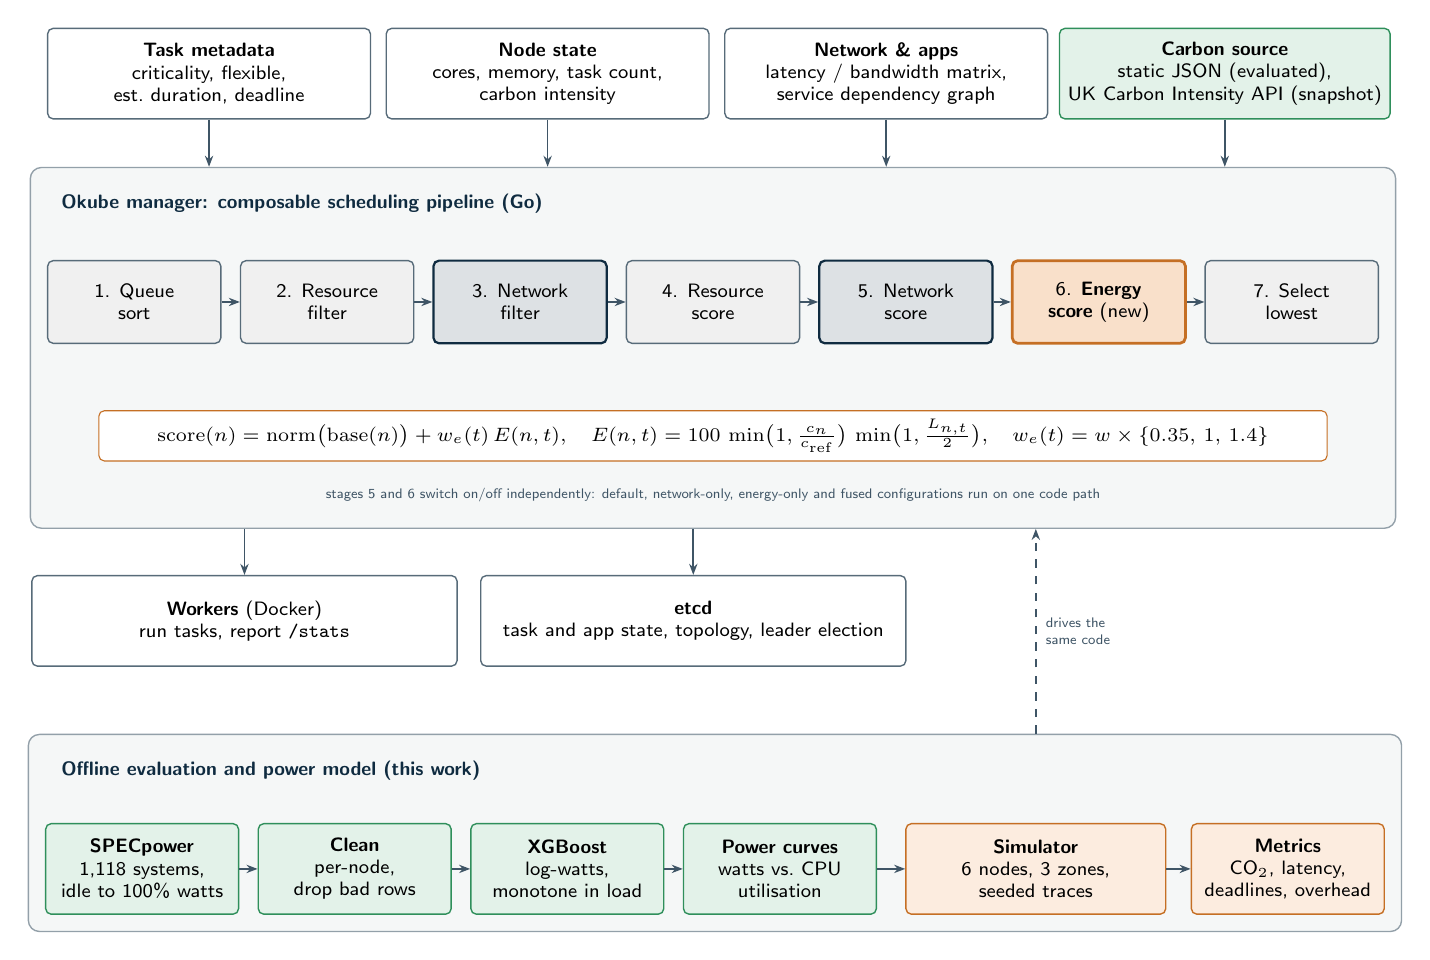
\begin{tikzpicture}[
  font=\sffamily\scriptsize,
  box/.style={draw=navy!70, rounded corners=2pt, fill=white, align=center,
              inner sep=3pt, line width=0.5pt, minimum height=1.15cm},
  stage/.style={box, fill=gray!12, minimum width=2.2cm, minimum height=1.05cm},
  netstage/.style={stage, fill=navy!14, draw=navy, line width=0.8pt},
  enstage/.style={stage, fill=okorange!25, draw=okorange!85!black, line width=1.0pt},
  cont/.style={draw=navy!45, rounded corners=4pt, inner sep=6pt, fill=navy!4, line width=0.5pt},
  arr/.style={-{Stealth[length=4pt]}, line width=0.6pt, navy!80},
  darr/.style={arr, dashed},
  title/.style={font=\sffamily\bfseries\scriptsize, navy, anchor=west},
]
% ---- inputs -----------------------------------------------------------------
\node[box, minimum width=4.1cm] (in1) at (2.15,10.2)  {\textbf{Task metadata}\\criticality, flexible,\\est.\ duration, deadline};
\node[box, minimum width=4.1cm] (in2) at (6.45,10.2)  {\textbf{Node state}\\cores, memory, task count,\\carbon intensity};
\node[box, minimum width=4.1cm] (in3) at (10.75,10.2) {\textbf{Network \& apps}\\latency / bandwidth matrix,\\service dependency graph};
\node[box, minimum width=4.1cm, fill=mint, draw=okgreen] (in4) at (15.05,10.2) {\textbf{Carbon source}\\static JSON (evaluated),\\UK Carbon Intensity API (snapshot)};

% ---- scheduling pipeline -----------------------------------------------------
\node[stage]    (s1) at (1.2,7.3)   {1. Queue\\sort};
\node[stage]    (s2) at (3.65,7.3)  {2. Resource\\filter};
\node[netstage] (s3) at (6.1,7.3)   {3. Network\\filter};
\node[stage]    (s4) at (8.55,7.3)  {4. Resource\\score};
\node[netstage] (s5) at (11.0,7.3)  {5. Network\\score};
\node[enstage]  (s6) at (13.45,7.3) {6. \textbf{Energy}\\\textbf{score} (new)};
\node[stage]    (s7) at (15.9,7.3)  {7. Select\\lowest};
\foreach \a/\b in {s1/s2,s2/s3,s3/s4,s4/s5,s5/s6,s6/s7}{\draw[arr] (\a) -- (\b);}
\node[title] (ptitle) at (0.15,8.55) {Okube manager: composable scheduling pipeline (Go)};
\node[align=center, fill=white, draw=okorange!85!black, rounded corners=2pt, inner sep=3pt, minimum width=15.6cm] (form) at (8.55,5.6)
  {$\mathrm{score}(n)=\mathrm{norm}\big(\mathrm{base}(n)\big)+w_e(t)\,E(n,t),\quad
    E(n,t)=100\,\min\!\big(1,\tfrac{c_n}{c_{\mathrm{ref}}}\big)\,\min\!\big(1,\tfrac{L_{n,t}}{2}\big),\quad
    w_e(t)=w\times\{0.35,\,1,\,1.4\}$};
\node[align=center, font=\sffamily\tiny, text=navy!80] (toggle) at (8.55,4.85)
  {stages 5 and 6 switch on/off independently: default, network-only, energy-only and fused configurations run on one code path};
\begin{scope}[on background layer]
  \node[cont, fit=(s1)(s7)(ptitle)(form)(toggle)] (pipe) {};
\end{scope}

% ---- cluster ------------------------------------------------------------------
\node[box, minimum width=5.4cm] (workers) at (2.6,3.25) {\textbf{Workers} (Docker)\\run tasks, report \texttt{/stats}};
\node[box, minimum width=5.4cm] (etcd)    at (8.3,3.25) {\textbf{etcd}\\task and app state, topology, leader election};
\foreach \n in {in1,in2,in3,in4}{\draw[arr] (\n.south) -- (\n.south |- pipe.north);}
\draw[arr] (workers.north |- pipe.south) -- (workers.north);
\draw[arr] (etcd.north |- pipe.south) -- (etcd.north);

% ---- offline evaluation and power model ------------------------------------------
\node[box, minimum width=2.45cm, fill=mint, draw=okgreen] (e1) at (1.3,0.1) {\textbf{SPECpower}\\1{,}118 systems,\\idle to 100\% watts};
\node[box, minimum width=2.45cm, fill=mint, draw=okgreen] (e2) at (4.0,0.1) {\textbf{Clean}\\per-node,\\drop bad rows};
\node[box, minimum width=2.45cm, fill=mint, draw=okgreen] (e3) at (6.7,0.1) {\textbf{XGBoost}\\log-watts,\\monotone in load};
\node[box, minimum width=2.45cm, fill=mint, draw=okgreen] (e4) at (9.4,0.1) {\textbf{Power curves}\\watts vs.\ CPU\\utilisation};
\node[box, minimum width=3.3cm, fill=okorange!15, draw=okorange!85!black] (e5) at (12.65,0.1) {\textbf{Simulator}\\6 nodes, 3 zones,\\seeded traces};
\node[box, minimum width=2.45cm, fill=okorange!15, draw=okorange!85!black] (e6) at (15.85,0.1) {\textbf{Metrics}\\CO$_2$, latency,\\deadlines, overhead};
\foreach \a/\b in {e1/e2,e2/e3,e3/e4,e4/e5,e5/e6}{\draw[arr] (\a) -- (\b);}
\node[title] (etitle) at (0.15,1.35) {Offline evaluation and power model (this work)};
\begin{scope}[on background layer]
  \node[cont, fit=(e1)(e6)(etitle)] (evalc) {};
\end{scope}
\draw[darr] (e5.north |- evalc.north) -- (e5.north |- pipe.south)
  node[midway, right, align=left, font=\sffamily\tiny, text=navy!80] {drives the\\same code};
\end{tikzpicture}
}
\caption{Architecture of Okube-Energy. Four inputs feed a seven-stage scheduling pipeline in the manager; stages 5 and 6 (network and energy score) are independently switchable. The bottom panel is the offline path: SPECpower data is cleaned and used to train a power model, whose curves let the simulator compute CO$_2$ while driving the same pipeline code.}
\label{fig:arch}
\end{figure*}

\textbf{Pipeline.} Scheduling is an ordered sequence of plugin stages mirroring the Kubernetes Scheduling Framework but implemented natively: (1) \emph{queue sort}, a topological sort so that a service is placed after its dependencies; (2) a \emph{resource filter}; (3) a \emph{network filter} that rejects nodes violating a hard per-edge latency or bandwidth constraint; (4) a \emph{resource score}; (5) a \emph{network score}; (6) the \emph{energy score} added in this work; and (7) selection of the lowest fused score. Stages 5 and 6 are skipped independently through a score context, which is what lets one implementation serve all four evaluated configurations.

\textbf{Metadata.} Tasks carry a criticality, a flexibility flag, an estimated duration and a deadline, which can be set in a deployment manifest. Nodes carry a carbon intensity, and the manager derives load from the number of running tasks and each worker's reported capacity. Carbon intensity is read from a JSON file keyed by worker; \texttt{scripts/fetch\_uk\_carbon.py} writes that file from the UK Carbon Intensity API.

% ---------------------------------------------------------------- IV. Scoring model
\section{Scoring Model}
\label{sec:model}
For a task $t$ and a candidate node $n$, scores are costs: lower is better.

\textbf{Network cost.} For a service $s$ in an application group, the network cost of $n$ is the summed latency to the nodes hosting $s$'s dependencies,
\begin{equation}
\mathrm{cost}_{\mathrm{net}}(n)=\sum_{e\in\mathrm{deps}(s)}\mathrm{latency}\big(n,\mathrm{node}(e.\mathrm{to})\big).
\label{eq:net}
\end{equation}
Network and resource costs are each min--max normalised to $[0,100]$ across the candidates and combined with weights $0.7$ and $0.3$:
\begin{equation}
\mathrm{base}(n)=0.7\,\mathrm{norm}\big(\mathrm{cost}_{\mathrm{net}}(n)\big)+0.3\,\mathrm{norm}\big(\mathrm{cost}_{\mathrm{res}}(n)\big).
\label{eq:base}
\end{equation}
Without topology or dependency data this stage is a no-op and the resource score passes through, so the scheduler degrades gracefully.

\textbf{Carbon cost.} Let $c_n$ be the node's carbon intensity as a unitless factor ($\mathrm{gCO_2/kWh}/1000$) and $L_{n,t}$ a load multiplier,
\begin{equation}
L_{n,t}=1+\frac{\mathrm{mem}(t)}{\mathrm{mem}(n)}+\frac{\mathrm{cpu}(t)}{\mathrm{cores}(n)}+0.08\,\mathrm{tasks}(n).
\label{eq:load}
\end{equation}
The energy cost is measured on a fixed 0--100 scale,
\begin{equation}
E(n,t)=100\,\min\!\Big(1,\frac{c_n}{c_{\mathrm{ref}}}\Big)\,\min\!\Big(1,\frac{L_{n,t}}{L_{\mathrm{ref}}}\Big),
\label{eq:energy}
\end{equation}
with $c_{\mathrm{ref}}=0.3$ (300\,g/kWh, about the dirty end of Great Britain's regional values) and $L_{\mathrm{ref}}=2$. A node with unknown intensity falls back to a default factor of $0.5$; a known intensity of $0$ costs nothing.

\textbf{Class-aware fusion.} The carbon weight is a base weight $w$ scaled by the task's class,
\begin{equation}
w_e(t)=w\times\begin{cases}0.35 & \text{critical or urgent}\\ 1.4 & \text{flexible}\\ 1 & \text{otherwise,}\end{cases}
\label{eq:weight}
\end{equation}
and the fused score, minimised over candidates, is
\begin{equation}
\mathrm{score}(n)=\mathrm{norm}\big(\mathrm{base}(n)\big)+w_e(t)\,E(n,t).
\label{eq:fused}
\end{equation}
The incoming scores are normalised so that $w$ means the same whether they came from the network stage or, without topology data, from raw resource costs.

\textbf{Properties.} (i) $w=0$ returns the incoming scores untouched, so the network-only baseline is exact. (ii) Because $E$ uses a fixed scale, three grids at $0$, $4$ and $15$\,g/kWh differ by less than $3$ points, whereas the normalised form scored them $0$, $27$ and $100$; a real spread of $0$, $100$ and $237$\,g/kWh differs by about $40$ points at idle load. (iii) Intensities above $c_{\mathrm{ref}}$ saturate, so two very dirty grids tie and the scheduler does not chase differences that no longer matter. Each property is covered by a unit test.

% ---------------------------------------------------------------- V. Data and power model
\section{Data and Power Model}
\label{sec:data}
\subsection{SPECpower\_ssj2008}
SPEC publishes, for every accepted result, the hardware configuration and the average active power at ten target loads from 10\% to 100\% and at active idle. We read the public results summary and then each result's detail page, respecting the site's requested crawl delay, which gave \NSystemsScraped{} systems with complete eleven-point curves (published \YearLo--\YearHi). Systems with several nodes report whole-system power and hardware, so cores, chips, threads, memory and watts are divided by the node count. After dropping three systems with missing values (no system had idle power above full-load power or non-rising power), \NSystemsKept{} systems and \NRowsKept{} (system, load) rows remain.

\subsection{Model}
Utilisation is taken as the target load. The features are utilisation, chips, cores, threads, clock frequency, memory, publication year, cores per chip, threads per core and memory per core. We fit XGBoost \cite{chen2016} (400 trees, depth 4, learning rate 0.05, row subsampling 0.8) to $\log(\mathrm{watts})$, with a monotone constraint that predicted power cannot fall as utilisation rises. Evaluation is by held-out \emph{system}, so no system appears in both train and test, in two ways: five-fold grouped cross-validation, and a temporal split that trains on systems published up to 2022 (\TrainSystems) and tests on later ones (\TestSystems).

\begin{table}[t]
\centering
\caption{Held-out error in watts per node (MAE) and percent (MAPE).}
\label{tab:power}
\footnotesize
\setlength{\tabcolsep}{3pt}
\begin{tabular}{@{}lrrrr@{}}
\toprule
 & \multicolumn{2}{c}{Grouped CV} & \multicolumn{2}{c}{Temporal split} \\
\cmidrule(lr){2-3}\cmidrule(lr){4-5}
Model & MAE & MAPE & MAE & MAPE \\
\midrule
Placeholder line (100--250\,W) & 142.5 & 65.1 & 250.8 & 65.9 \\
Line through true idle/max (oracle) & 20.5 & 7.7 & 33.7 & 8.2 \\
Ridge regression & 75.7 & 32.9 & 205.1 & 46.2 \\
XGBoost (ours) & 32.7 & 12.0 & 118.0 & 25.8 \\
\bottomrule
\end{tabular}

\end{table}

Table~\ref{tab:power} shows that the model reduces the error of the placeholder line from \MapePlaceholder\% to \MapeXgb\%. A straight line through each system's true idle and full-load watts has only \MapeOracle\% error, so a line between those two points is a good description of a real curve, and the extra error of the model comes from not knowing the idle and peak of a specific machine. Error on newer hardware is larger (\MapeTemporal\% on the temporal split). Figure~\ref{fig:power} shows the predicted curves for the node types used here. For an 8-core single-socket node the model predicts \SmallIdle{}\,W idle, \SmallHalf{}\,W at half load and \SmallPeak{}\,W at full load, against a median of 20, 44 and 81\,W for 34 comparable real systems from 2019 or later.

\begin{figure}[t]
\centering
\begin{tikzpicture}
\begin{axis}[width=\columnwidth, height=5.0cm, xlabel={CPU utilisation}, ylabel={Power (W)},
  xmin=0, xmax=1, ymin=0, grid=major, grid style={gray!25}, tick label style={font=\footnotesize},
  label style={font=\footnotesize}, legend style={font=\scriptsize, at={(0.02,0.98)}, anchor=north west},
  legend cell align=left]
\addplot[thick, navy, mark=*, mark size=1.2pt] table[x=u, y=small] {generated/power_curves.dat};
\addlegendentry{8 cores, 32\,GB (used)}
\addplot[thick, okgreen, mark=square*, mark size=1.2pt] table[x=u, y=mid] {generated/power_curves.dat};
\addlegendentry{32 cores, 128\,GB}
\addplot[thick, okorange, mark=triangle*, mark size=1.5pt] table[x=u, y=large] {generated/power_curves.dat};
\addlegendentry{64 cores, 256\,GB}
\addplot[thick, dashed, gray!70!black] table[x=u, y=placeholder] {generated/power_curves.dat};
\addlegendentry{old placeholder (8 cores)}
\end{axis}
\end{tikzpicture}
\caption{Power curves predicted by the model for three hardware profiles, and the 100--250\,W placeholder it replaces.}
\label{fig:power}
\end{figure}

\subsection{UK Carbon Intensity API}
The Carbon Intensity API \cite{carbonapi} is operated by NESO with the University of Oxford, EDF Europe and WWF, is licensed CC~BY~4.0, and needs no key. Its regional endpoint returns the current half-hour's indicative intensity for each of Great Britain's regions (and national aggregates), and a forecast is available. On 23 October 2026 the regional values spanned $0$ (North Scotland) to $237$\,g/kWh (South Wales). We use it in two ways. First, \texttt{scripts/fetch\_uk\_carbon.py} converts a regional snapshot into the \texttt{carbon\_intensity.json} the manager loads, and a test checks that file loads with a real zero preserved; a snapshot taken on 24 October 2026 read $0$, $5$ and $137$\,g/kWh for North Scotland, North West England and South Wales. Second, those magnitudes calibrated the \emph{illustrative} intensities of the simulated zones (Section~\ref{sec:eval}). The simulation does not consume the live feed, and continuous refresh is future work.

% ---------------------------------------------------------------- VI. Evaluation method
\section{Evaluation Method}
\label{sec:eval}
\textbf{Simulator.} A deterministic simulator drives the real scheduler pipeline (filter, score, select) with an event loop: arrivals are scheduled, tasks occupy cores and memory until they finish, a task waits if no node has room, and a service waits for its dependencies to be placed. It uses an offline, deterministic least-loaded resource scorer so that decisions do not depend on call order or on live worker statistics.

\textbf{Scenario.} Six nodes of 8 cores and 32\,GiB in three zones of two nodes: \texttt{scot} (50\,g/kWh), \texttt{nw} (180) and \texttt{south} (260). Latency is 2\,ms within a zone and 12, 10 and 22\,ms between \texttt{scot}--\texttt{nw}, \texttt{nw}--\texttt{south} and \texttt{scot}--\texttt{south}. The cleanest zone is thus the farthest from the dirtiest, so latency-driven and carbon-driven placements disagree. The intensities are illustrative UK-like values, not measurements. Every node uses the learned 8-core curve.

\textbf{Workloads.} A trace is a seeded sequence of application deployments drawn from three templates (a four-service shop, a three-service analytics job and a three-service media pipeline). The \emph{default} workload has 60 deployments with a mean inter-arrival of 75\,s, sized for about 35\% average utilisation, so that nodes have room and the scheduler has a choice. Each deployment is critical, flexible or default with probability 0.2, 0.4 and 0.4, runs 60--600\,s, and has a deadline 1.5, 6 or 3 times its duration after arrival. The \emph{stress} workload arrives 2.5 times faster and saturates the cluster.

\textbf{Configurations and metrics.} The four configurations are default (stages 5 and 6 off), network-only (6 off), energy-only (5 off) and fused. Network-off configurations also withhold the topology from the hard network filter, so they are genuinely network-blind. We report (i) \emph{dynamic CO$_2$}: each node's power above idle, read from its curve at the actual utilisation and integrated over time, shared among the running tasks by CPU request, and multiplied by the node's intensity; (ii) mean \emph{dependency latency}, Eq.~\eqref{eq:net} for services that have dependencies; (iii) the deadline-violation rate; and (iv) the scheduling time per decision. Idle power is excluded from CO$_2$ because no placement avoids it.

\textbf{Protocol.} Within a seed every configuration sees the identical trace, so differences are paired. We chose the energy weight on seeds 1--30 as the largest $w$ for which mean latency stays within 10\% of network-only and the violation rate does not rise on both workloads, which gives $w=\HeadlineW$. All results below come from the disjoint seeds 101--150 (\NSeeds{} runs per cell). Intervals are 95\% confidence intervals on the paired mean, $1.96\,s/\sqrt{n}$.

% ---------------------------------------------------------------- VII. Results
\section{Results}
\label{sec:results}
Table~\ref{tab:results} gives the main comparison. At the scheduler's default weight of 0.2 the fused scheduler already cuts CO$_2$ by \FusedLowW\% against the default scheduler while network-only cuts it by only \NetCO\%. At the selected weight of \HeadlineW{} the fused scheduler cuts it by \FusedCO\% ($\pm\FusedCOci$) and keeps latency \FusedLatCut\% below default, close to the \NetLatCut\% of network-only. The energy-only scheduler at the same weight reaches \EnergyOnlyCO\% with a latency reduction of only about 20\%.

\begin{table*}[t]
\centering
\caption{Dynamic CO$_2$ (g per run, mean over \NSeeds{} seeds) and mean dependency latency. $\Delta$ is the paired change against the default scheduler; CO$_2$ changes carry a 95\% confidence interval. Rows below the rule use the selected weight.}
\label{tab:results}
\footnotesize
\setlength{\tabcolsep}{4pt}
\begin{minipage}[t]{0.49\textwidth}
\centering\textbf{Default workload}\\[2pt]
\begin{tabular}{@{}llrrrr@{}}
\toprule
Config & $w$ & CO$_2$ & $\Delta$CO$_2$ (\%) & Lat.\ (ms) & $\Delta$Lat.\ (\%) \\
\midrule
Default & -- & 25.66 & -- & 13.62 & -- \\
Network-only & -- & 25.20 & $-1.7\ \pm0.9$ & 2.26 & $-83.3$ \\
Energy-only & 0.2 & 24.91 & $-2.8\ \pm0.8$ & 11.82 & $-12.9$ \\
Fused & 0.2 & 24.32 & $-5.2\ \pm1.1$ & 2.09 & $-84.6$ \\
\midrule
Energy-only & 1.5 & 23.77 & $-7.3\ \pm0.8$ & 10.84 & $-20.2$ \\
Fused & 1.5 & 22.34 & $-12.9\ \pm1.2$ & 2.57 & $-81.0$ \\
\bottomrule
\end{tabular}

\end{minipage}\hfill
\begin{minipage}[t]{0.49\textwidth}
\centering\textbf{Stress workload}\\[2pt]
\begin{tabular}{@{}llrrrr@{}}
\toprule
Config & $w$ & CO$_2$ & $\Delta$CO$_2$ (\%) & Lat.\ (ms) & $\Delta$Lat.\ (\%) \\
\midrule
Default & -- & 24.51 & -- & 12.99 & -- \\
Network-only & -- & 24.48 & $-0.1\ \pm0.6$ & 5.62 & $-56.5$ \\
Energy-only & 0.2 & 24.36 & $-0.6\ \pm0.5$ & 12.01 & $-7.3$ \\
Fused & 0.2 & 24.24 & $-1.1\ \pm0.6$ & 5.52 & $-57.2$ \\
\midrule
Energy-only & 1.5 & 23.97 & $-2.2\ \pm0.6$ & 11.17 & $-13.6$ \\
Fused & 1.5 & 23.91 & $-2.4\ \pm0.7$ & 5.98 & $-53.7$ \\
\bottomrule
\end{tabular}

\end{minipage}
\end{table*}

\begin{figure}[t]
\centering
\begin{tikzpicture}
\begin{axis}[width=\columnwidth, height=5.6cm, xlabel={Mean dependency latency (ms)},
  ylabel={CO$_2$ reduction vs.\ default (\%)}, xmin=1.5, xmax=14.5, ymin=-3, ymax=46,
  grid=major, grid style={gray!25}, tick label style={font=\footnotesize}, label style={font=\footnotesize},
  legend style={font=\scriptsize, at={(0.98,0.97)}, anchor=north east}, legend cell align=left,
  every node near coord/.append style={font=\scriptsize, inner sep=1.5pt}]
\addplot[thick, okorange, mark=*, mark size=1.3pt] table[x=lat, y=red] {generated/sweep_fused_default.dat};
\addlegendentry{fused, $w=0..10$}
\addplot[thick, okgreen, mark=square*, mark size=1.3pt] table[x=lat, y=red] {generated/sweep_energyonly_default.dat};
\addlegendentry{energy-only, $w=0..10$}
\addplot[only marks, mark=diamond*, mark size=3pt, navy] table[x=lat, y=red] {generated/points_default.dat};
\addlegendentry{default / network-only}
\addplot[only marks, mark=*, mark size=1.3pt, okorange, nodes near coords, point meta=explicit symbolic, every node near coord/.append style={anchor=west, xshift=2pt, text=okorange!70!black}] table[x=lat, y=red, meta=label] {generated/labels_fused_default.dat};
\addplot[only marks, mark=square*, mark size=1.3pt, okgreen, nodes near coords, point meta=explicit symbolic, every node near coord/.append style={anchor=south west, text=okgreen!60!black}] table[x=lat, y=red, meta=label] {generated/labels_energyonly_default.dat};
\end{axis}
\end{tikzpicture}
\caption{Carbon--latency trade-off over the energy weight $w$ (default workload; labels give $w$). Diamonds mark the default scheduler (right) and network-only (left).}
\label{fig:tradeoff}
\end{figure}

\textbf{Trade-off.} Figure~\ref{fig:tradeoff} traces the weight sweep. The fused curve stays far to the left of the energy-only curve: for the same carbon reduction it pays a fraction of the latency. Raising $w$ further buys more carbon (about 35\% at $w=5$) for progressively more latency, which is the trade-off the weight exposes, and our 10\% latency budget is a judgement: a looser budget would select a larger weight.

\textbf{Task classes.} Table~\ref{tab:class} shows the mean grid intensity of the nodes each class ran on. With class-aware weights, flexible tasks move to cleaner nodes ($119$\,g/kWh at the selected weight, against $162$ for the default scheduler), while critical tasks move the other way ($183$\,g/kWh) because flexible work takes the clean capacity.

\begin{table}[t]
\centering
\caption{Mean grid intensity (g/kWh) of the nodes used, by task class (default workload).}
\label{tab:class}
\footnotesize
\begin{tabular}{@{}lrr@{}}
\toprule
Config & Flexible & Critical \\
\midrule
Default & 162 & 161 \\
Network-only & 161 & 164 \\
Energy-only ($w{=}1.5$) & 133 & 170 \\
Fused ($w{=}1.5$) & 119 & 183 \\
\bottomrule
\end{tabular}

\end{table}

\textbf{Stress workload.} When the cluster is saturated only one or two nodes have room for each task, and the scheduler has little to choose. Carbon gains fall to \FusedCOStress\% at the selected weight, and the latency reduction is smaller (\FusedLatCutStress\% below default, against \NetLatCutStress\% for network-only).

\textbf{Deadlines and overhead.} Deadline-violation rates do not differ between configurations (about 0.03\% on the default workload and 2.4--2.6\% under stress), so energy-awareness at these weights does not cost deadlines, but our deadlines do not separate the schedulers either. A fused scheduling decision takes about \FusedDecisionUs\,$\mu$s with the offline scorer, against under one microsecond for the default scheduler; with the EPVM scorer it would be dominated by its worker-statistics calls.

% ---------------------------------------------------------------- VIII. Discussion
\section{Discussion and Threats to Validity}
\label{sec:discussion}
\label{sec:threats}
\textbf{The comparison with energy-only is not a pure test of fusion.} In the fused scheduler the resource term is weighted $0.3$ by the network stage; in energy-only, with the network stage off, the resource score passes through unweighted. The energy term therefore competes against a weaker load-balancing term in the fused scheduler, and part of fused's lead over energy-only is this reweighting and not synergy between network and carbon. A like-for-like comparison would give energy-only the same resource weight.

\textbf{The learned model does not influence placement.} Scheduling decisions use the heuristic of Eq.~\eqref{eq:energy}; the power model only converts placements into CO$_2$. We therefore do not claim a scheduler driven by predicted energy, and only that CO$_2$ is computed from a model grounded in measured data.

\textbf{Carbon data are illustrative, and static.} Zone intensities are UK-like magnitudes, not measurements, and are constant through each run. Absolute CO$_2$ is a relative comparison between schedulers, not a real emission. Static intensities also remove the largest real lever, running work when the grid is clean, which we do not implement.

\textbf{Power model limits.} A single non-federated model; identical hardware in every node, so the scheduler cannot exploit efficiency differences; target load stands in for CPU utilisation; and error of \MapeXgb\% on held-out systems and \MapeTemporal\% on newer ones. Systems with the same chips and cores differ by factors of two or three in watts, which no feature here explains.

\textbf{Simulation scope.} Latency is the topological cost of Eq.~\eqref{eq:net}, not measured request latency; the weight was tuned and the results reported on different seeds but the \emph{same} scenario and workload generator, so generalisation to other clusters is untested; and no live cluster run backs the numbers.

\textbf{Side effects.} At high weights critical tasks end on dirtier nodes (Table~\ref{tab:class}); and dynamic CO$_2$ excludes idle power, which is \IdleShare\% of total CO$_2$ on the default workload (\IdleShareStress\% under stress). Consolidating work so idle nodes can be powered down is a lever we do not model.

% ---------------------------------------------------------------- IX. Conclusion
\section{Conclusion}
We extended Okube with a single scheduling pipeline in which network and carbon costs are independent, class-aware stages. A fixed-scale carbon cost, a power model learned from \NSystemsKept{} real systems, and a paired, held-out evaluation support a specific claim: on a three-zone simulated cluster the fused scheduler at an energy weight of \HeadlineW{} reduces dynamic CO$_2$ by \FusedCO\% over the default scheduler while keeping latency \FusedLatCut\% below default, a combination neither the network-only nor the energy-only scheduler reaches. The claim comes with clear limits: illustrative carbon data, one hardware type, a saturated-load regime where the gain largely vanishes, and a comparison to energy-only that is partly a reweighting effect.

% ---------------------------------------------------------------- X. Future work
\section{Future Work}
\label{sec:future}
\begin{itemize}
\item \textbf{Live carbon feed.} Refresh intensities continuously from the UK Carbon Intensity API, keeping the static file as an offline fallback, and evaluate on a multi-region deployment.
\item \textbf{Temporal placement.} Use the API's forecast to delay flexible jobs with deadline slack into cleaner windows, adding \emph{when} to \emph{where}.
\item \textbf{Predicted energy in the score.} Feed the marginal watts of a placement from the power model into Eq.~\eqref{eq:energy}, which also matters once nodes differ in hardware.
\item \textbf{Federated power model.} Train per-partition models and merge them, as in \cite{saad2025}, and compare with the single model here.
\item \textbf{Fair ablation and live runs.} Give energy-only the same resource weight as fused, and validate the simulator against a real multi-worker cluster.
\item \textbf{Kubernetes port.} Reimplement the filter and score stages as a Scheduling Framework plugin once the design is stable.
\end{itemize}

\section*{Acknowledgment}
The authors would like to express their sincere gratitude to the Department of Information Technology, NITK Surathkal, for providing continuous support and guidance throughout this project, and to our guide, Dr.\ Bhawana Rudra. We also thank our mentors and peers for their valuable feedback during the development phase.

\begin{thebibliography}{99}
\bibitem{santos2023} J. Santos, C. Wang, T. Wauters, and F. De Turck, ``Diktyo: Network-aware scheduling in container-based clouds,'' \emph{IEEE Trans.\ Netw.\ Service Manag.}, vol.~20, no.~4, pp.~4461--4477, 2023, doi: 10.1109/TNSM.2023.3271415.
\bibitem{saad2025} Z. Saad, J. Yang, H. Leung, and S. Drew, ``Towards carbon-aware container orchestration: Predicting workload energy consumption with federated learning,'' in \emph{Proc.\ IEEE Smart World Congress (SWC)}, 2025, arXiv:2510.03970.
\bibitem{piontek2024} T. Piontek, K. Haghshenas, and M. Aiello, ``Carbon emission-aware job scheduling for Kubernetes deployments,'' \emph{J.\ Supercomput.}, vol.~80, pp.~549--569, 2024, doi: 10.1007/s11227-023-05506-7.
\bibitem{amaral2023} M. Amaral \emph{et al.}, ``Kepler: A framework to calculate the energy consumption of containerized applications,'' in \emph{Proc.\ IEEE Int.\ Conf.\ Cloud Computing (CLOUD)}, 2023.
\bibitem{survey2025} ``A survey on task scheduling in carbon-aware container orchestration,'' arXiv:2508.05949, Aug.\ 2025.
\bibitem{lange2009} K.-D. Lange, ``Identifying shades of green: The SPECpower benchmarks,'' \emph{Computer}, vol.~42, no.~3, pp.~95--97, 2009. Results: \url{https://www.spec.org/power_ssj2008/results/}, accessed Oct.\ 2026.
\bibitem{carbonapi} National Energy System Operator (NESO) with the University of Oxford, EDF Europe and WWF, ``Carbon Intensity API,'' \url{https://carbonintensity.org.uk}, CC BY 4.0, accessed Oct.\ 2026.
\bibitem{chen2016} T. Chen and C. Guestrin, ``XGBoost: A scalable tree boosting system,'' in \emph{Proc.\ ACM SIGKDD}, 2016, pp.~785--794.
\end{thebibliography}

\end{document}
